\documentclass[sigconf]{acmart}

\usepackage{booktabs} % For formal tables


\setcopyright{rightsretained}



% DOI
\acmDOI{10.475/123_4}

% ISBN
\acmISBN{123-4567-24-567/08/06}

%Conference
\acmConference[WOODSTOCK'97]{ACM Woodstock conference}{July 1997}{El
  Paso, Texas USA} 
\acmYear{1997}
\copyrightyear{2016}


\acmArticle{4}
\acmPrice{15.00}

% These commands are optional
%\acmBooktitle{Transactions of the ACM Woodstock conference}
%\editor{Jennifer B. Sartor}
%\editor{Theo D'Hondt}
%\editor{Wolfgang De Meuter}


\begin{document}
\title{Automating State to State testing of mobile applications to mobile platforms}
\titlenote{Produces the permission block, and
  copyright information}
\subtitle{Edition 1}
\subtitlenote{The full version of the author's guide is available as
  \texttt{acmart.pdf} document}


\author{Jonathan Sanders}
%\authornote{Dr.~Trovato insisted his name be first.}
%\orcid{1234-5678-9012}
%\affiliation{%
%  \institution{Institute for Clarity in Documentation}
%  \streetaddress{P.O. Box 1212}
%  \city{Dublin} 
%  \state{Ohio} 
%  \postcode{43017-6221}
%}
%\email{trovato@corporation.com}

\author{Dr. Justice}
%\authornote{The secretary disavows any knowledge of this author's actions.}
%\affiliation{%
%  \institution{Institute for Clarity in Documentation}
%  \streetaddress{P.O. Box 1212}
%  \city{Dublin} 
%  \state{Ohio} 
%  \postcode{43017-6221}
%}
%\email{webmaster@marysville-ohio.com}


% The default list of authors is too long for headers.
\renewcommand{\shortauthors}{B. Trovato et al.}


\begin{abstract}
This paper outlines a new way to test a devices states' affect on an application.  
\end{abstract}



\keywords{automata for mobile device testing,automated state testing}


\maketitle

\section{Introduction}
\subsection{Overview}
Android applications have become a staple of many people's everyday mobile computing user experience.  As of the first quarter of 2017 Android possessed 85\% of the mobile phone market \cite{chau_2017}.  The need for complete and thorough testing capabilities of Android applications has never been greater. There is currently a deficit in an area of testing for mobile devices regarding the "state" of the mobile device while testing is taking place. Very often, particular states will cause a failure of a mobile application and currently there are not any good tools available to test different states to avoid these types of failures.
\begin{figure}[t]
	\centering
	\caption[TADS work flow]{TADS work flow (contents of a DSC)}
	\label{fig:table1}
	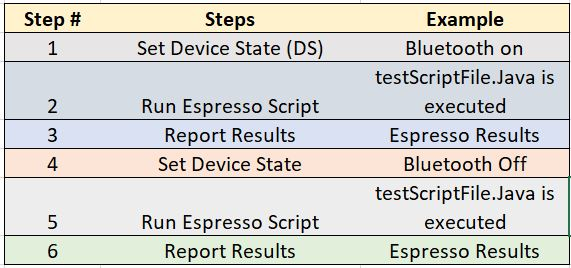
\includegraphics[width=1\linewidth]{table1}
\end{figure}
The state of the device is the current settings of different modules within the mobile device such as if bluetooth is on or off or if airplane mode is on or off; other "states" include having different applications running that access common instrumentation or having hardware devices connected to the mobile device and running with an application such as a heart rate monitoring application running with a conected physical Electrocardiogram (EKG).  Any configuration of these different instruments, applications, operating system configurations, or modules can be considered a device's state; hereto referred as Ds for device state.

We have developed a novel approach to very easily run existing Android test scripts against any Ds one could imagine.  The solution we built is called "TADS" (Testing Application to Device State) that uses Espresso, an automated Android application testing tool, to test the Mobile application against multiple DSs.  TADS is primarily concerned with identifying errors caused by changing device states and not as concerned with identifying why the state change caused a failure; error checking is already provided by Espresso scripts.  TADS does show which TADS test failed.

Espresso is a tool developed by Google that enables a user to easily record a series of events, then create an oracle (an oracle is a way of knowing if the series of events executed correctly) so that the user can create an automated test case.  The Espresso recorder autmatically generates a testing script that can be executed at any time to recreate the series of events and check the oracle to ensure the series of events executed correctly.  The script then generates a pass or fail message that the user can see to know if any recent development work broke the existing software application. 

TADS uses a simple principle of looping through various DSs.  Figure 1. demonstrates the following process for testing. TADS will set a baseline DS, run the Espresso script, get the results, then change the DS, and then re-run the Espresso script and report those results.  A conglomuration of testing different DSs becomes a function in the TADS application called a Device State Change hereto referred as a DSC.  One example is the bluetooth DSC.  Bluetooth is turned on by TADS, the Espresso script is executed, then bluetooth is turned off by TADS, and lastly the Espresso script is executed and the results of that test are reported to the user.

It is more expensive for a company to not test applications against DSs because the failures are often catastrophic.  Companies have encountered these bugs after releasing an update for their application on the users' devices and the failure often causes a loss of credibility, loss of functionality that must then be quickly corrected and updated, and ultimately costs the company a loss of customers and money.  Testing the different states of just an application has been enhanced with tools such as Espresso, Barista, and Robotium \cite{optimusinformationinc2016} but the lack of testing those application states against the device state is where the problem lies.  Since the state of an application can be easily saved and the state of a device can be easily changed programmatically, a solution that automatically tests application states with different device states is of great value.  For applications being used in different device states, such as a "mapping" applications used outside of network range or medical applications using sensors for monitoring functions, application to device state testing becomes an extremely important issue.  Some of these issues can even be life safety critical.  One example is that of medical applications utilizing portable Electrocardiograms.  These devices are used to monitor a patient's heart rythems in order to detect anomolyes that are symptoms of particular life threatening diseases \cite{boulos2014mobile}.  If a Ds causes a small failure in the medical application, incorrect results can be reported resulting in a false positive or a false negative.  The innovative ways applications are used with new hardware is only increasing.  State testing of applications with new hardware devices is a critical area of research to ensure that applications can continue to operate well. 

An emerging field that is gaining tremendous traction in the mobile device industry where testing of DSs is absolutly critical is that of context aware applications.
According to Luo et al, there is a strong need for innovative approaches to testing context aware applications \cite{Luo:2017:TLT:3139486.3130945}. TADS is a innovative approach to do context aware testing. 

A "context aware" application is an application that is able to detect information about the device's physical environment using instrumentation and then do something with that information.  For instance, a context aware application can get GPS information and see that a user is at work, get location information from the network to see where in the building the user is, then get information from the calendar application about what is scheduled at that moment, and then the context aware application will determine that the user is in a board room in their office building during a scheduled meeting, and puts the phone on silent automatically or even stops all calls and replies with a text message saying the user is unavailable. Ds testing is critical for these types of applications.  If another application acccessing certain instrumentation information collides with the context aware applications access of that data, the context aware application will fail. Currently, there is not a way to determine if that will happen using common automated testing tools. 

\subsection{Research Contributions}
For our first contribution, as of the writing of this paper, there is not any research available about automatic device state testing.  Our work highlights and addresses this need directly and gives researchers and companies an option to pursue that enables them to create Ds testing with their Android applications.

The next main contribution of this work is that TADS demonstrates that a library for doing state testing of devices, that can be run with Espresso scripts, is highly beneficial and easy to make.  This research contributes a tool that can be used right now for anyone wanting to improve their test suites to include device state testing. The full source code can be seen and downloaded at: \url{https://github.com/UCCS-CS5371-Fall2017/jsander7/tree/master/ProjectFiles}.

Another contribution this work makes is that TADS also tackles a further research problem, presented by Fazzini et al. \cite{7927971}, of testing instrumentation in an automated fashion.  TADS extends Fazzini et al's work.  They highlight the fact that most instrumentation and Ds testing against an application is currently being done manually and that it is very time consuming and expensive because of the personnel hours required to complete that testing.  Fazzini et al. created Barista which is a better way to record and execute Android testing than Espresso.  Barista is an application that records user interactions with any Android application and automatically can generate oracles and then it records those interactions and oracles into an Espresso type script for later execution.  TADS can be easily integrated with Barista to enable the user to run Espresso scripts generated by Barista with different DSs.

The last contribution this work makes is a very simple way for testing context-aware applications' handling of instrumentation state changes. The work done by Luo et al \cite{Luo:2017:TLT:3139486.3130945} produces test data for context aware applications.  TADS tests the affect of changing the state of the instruments used by those applications.  A DSC can be easily generated that changes the states of the instruments that the context aware application uses in order to ensure changing instrumentation states will not cause a failure or worse, a false positive or false negative.

\section{Background}
TADS is built out of the Microsoft Powershell application.  TADS also utilizes the Android Device Bridge and Android Studio.  An overview of those are presented below.

Android Studio is Google's integrated development environment for developing Android applications.  Android studio generates a project when an Android application is started and within that project is a testing project.  When a developer makes an automated test those scripts are included in that test project.  Then, when the application is installed on a mobile device with the testing project attached (which is the default behavior of Android Studio, the test scripts are included on the device and can be executed via the Android Device Bridge.  

Espresso, an android testing application, is part of Android Studio and is an excellent tool for testing Mobile application UI's \cite{nolan2015agile}.  The tool records what is happening at a code level while a user performs different actions using the UI.  This enables a working application to have a test automatically generated that can then be run at a later time which can be used to create a regression test suite.  This actually enables states of the application to be tested without having to use any form of state machines or modeling.  This tool called "Test Recorder" is foundational to TADS.  When espresso scripts are stored in a test project within Android studio they becomes a test suite.  TADS can easily run an entire suite or an individual test script which is referred to as a test case.

"Android Debug Bridge, aka ADB, is a command-line utility included with Google's Android sdk. ADB can control your device over USB from a computer, copy files back and forth, install and un-install apps, run shell commands, and more." \cite{hoffman2017}  TADS relies heavily on the ADB. The ADB allows scripts to be run from a system other than the device itself either over a hard wire connection such as a USB connection from a computer to the device or over a network connection.  For some tests that TADS runs, a hardwire connection is required because at times the network connection is being tested and a hardwire connection is required when the network is turned off.  

TADS is developed in Microsoft Powershell.  Powershell is an enhanced version of the MSDos program.  Powershell includes the .NET runtime and libraries which enables a developer to leverege the tools that .NET provides.  There is a Powershell Integrated Development Environment called Windows Powershell ISE.  With ISE all of the results of executing an ADB command can be viewed and recorded if desired.  Powershell also has the ability to organize code into modules and plain Powershell scripting files.  The modules are suffixed with a file type of .psm1.  The normal script files are suffixed with the file type .ps1.  TADS is made up of many functions in several modules and Powershell files that execute ADB commands from a computer that the device is connected to.   


\section{Implementation}

\begin{figure}[h]
	\centering
	\caption[Public Interface]{Public Interface}
	\label{fig:table2}
	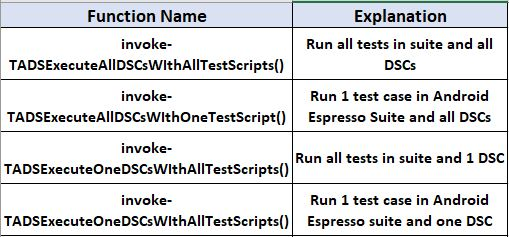
\includegraphics[width=1\linewidth]{table2}
\end{figure}

The main purpose of TADS is to simplify testing of different device states an Android application.  There are preloaded "device state changes" (DSCs) that can be used with a pre-made Espresso Test Script that are chosen for testing.  A DSC is a test case that starts with a device state then runs the test cases and then changes the Devices state, see Figure 1..  The DSC then runs the tests again with the new state set.  Another example of a DSC is: airplane mode off, run Espresso test script(s), switch airplane mode to on, then re-run the Espresso test script(s).

The implementation allows a user to call a function to test the following as is shown in Figure 1.  The user can run all of their test suites and all of the DSC's available, all tests and 1 DSC that is selected, 1 DSC and 1 test case in the suite, and all DSCs and 1 test case. The name of the application should be the whole app name starting with "com.".  The appropriate global variables should be filled in prior to calling the testing function. The public interface in Figure 1 is what novice programmers should use.

All of the files are available to be seen and modified.  New DSCs can be easily added using the idioms of the TADS solution in order to make very thorough test cases.

The TADS solution is built on Microsoft Powershell and written as Powershell scripts.  Powershell was decided on to enforce DRY and SOLID principles as much as possible without the convolution of building an executable program that is compiled.  DRY and SOLID principles are ways of writing code that is clean and easy to reuse.  

The TADS solution is run by executing a powershell script.  There are global variables that must be populated by the user to indicate several items.  Figure 2. demonstrates those global variables.  They are modified in the file called "Project Main.ps1"  The easiest way to execute TADS testing is via the Powershell ISE. 

Figure 2 is a break down of the functions to be called by your command line or in a script that a developer would write to test their application how they deem necessary.  The function applicable to what the developer is testing will be used.    

There is a readme.txt file that should be followed to get the testing environment set up for usage of the TADS solution and there are thorough instructions included in the readme.txt file.  The TADS solution can be downloaded at: \url{https://github.com/UCCS-CS5371-Fall2017/jsander7/tree/master/ProjectFiles} \\


\begin{figure}[t]
	\centering
	\caption[Contents of Files]{Contents of Files}
	\label{fig:table3}
	\includegraphics[width=1\linewidth]{table3}
\end{figure}

   

All functions in the entire solution are available to be consumed by the user.  This is so that a programmer can build their own Powershell script out of the existing functions and extend what has been made up to this point.  
As seen in Figure 3., within the TADS solution there are four main files.  They are: ProjectMain.ps1, DSCs.psm1, TestSuiteCommands.psm1, and ADBCommands.psm1.  The DSCs file contains all of the DSCs which is comprised of calls to the TestSuiteCommands and ADBCommands.  The TestSuiteCommands file contains the public interface found in Figure 1 and the commands that run the test suites in Espresso.  The ADMCommands file is where the state change commands are located that use ADB to change the states of the device. 



\section{Evaluation}
TADS has been able to run multiple tests against multiple DSs utilizing two DSCs.  The DSCs made are for bluetooth and airplane mode.  The bluetooh DSC turns bluetooth on, executes the test case generated, and then turns bluetooth off and executes the test case.  Airplane mode does the same for airplane mode.    

We utilized a recipe app for initial testing.  We recorded the selection of a recipe and the assertion was just verifying that recipe appeared.  The second test involved selecting a recipe, ensuring the recipe appears, and then going back to the home screen of the app and ensuring the recipe list appears.  

The recipe app was actually created for android wear as well.  TADS easily handled testing this application which connects to an android wear device.  

The results were simply passed tests.  We did not attempt to create any mutation tests by modifying code because the actual test is generated by the android test recorder Espresso.  

We evaluated the affectiveness of the application by adding code to the application that caused an exception to be thrown if bluetooth was off.  We did the same if wifi was turned off to create an exception so that the airplane mode tests would show that having one state passes and another state causes a failure of the application.  

These were simple tests but prove the idea that TADS demonstrates.  100% of the time these tests were caught.  Additionally, TADS adds test cases to be run.  Just two DSCs adds 4 test cases that are viable and valuable tests to be run.

\section{Related Work}
There are several tools developed that can capture various information of an application and store said information for later tests.  These tools can be leveraged to create interesting app states instead of simple object states.  For instance Paulovsky et al. \cite{7962332} built a tool that automatically captures UI information as a user utilizes an application. 

Many others, such as Fazzini et al \cite{7927971} have made tools for recording tests that can be later executed in ways that are platform independent which is a nice utility that we will not be concerned with in this work.  Others have made unit level state testing models such as MilaniFard el al. \cite{MilaniFard:2014:LET:2642937.2642991} in which the state of the application is tested by automatically building a model using a dynamic and static crawler and then running that created model against a verification algorithm.  Their work levereges data modeling to find issues device state whereas TADS utilizes real world scenarios executed on real world devices.  

G. Bai et al developed a way to use model testing to find security vulnerabilities \cite{7911333}.  Choi et al have used machine learning to find the states of an application that are probably of value to test that have not been tested and make a model of those states for testing \cite{Choi:2013:GGT:2544173.2509552}.  Their work could be applied by developers utilizing TADS to develop DSCs appropriate for their application type. \\


\section{Future Research}
A future research opportunity would be to implement the TADS solution in a way that the state changes can be called easily within an Espresso script.  That would enable knowledgeable testers to correctly evaluate the affect of different state changes on their solutions at specific times during execution of the script.   

Another challenge is that commands do not exist for ADB to change proprietary device instrumentation states.  Figuring out how to instantiate different hardware devices from the command interface and easily implement new DSCs will prove extremely beneficial in making robust state testing of Android applications using proprietary instrumentation suchh as a portable Electrocardiograms.  

Barista \cite{7927971} provides a better script generation tool than Espresso.  Integrating TADS to run Barista could prove to be a valuable endeavor.  Also, being able to inject DSCs into Barista generated testing scripts will enhance the ability of Barista to catch bugs introduced by device state changes.  

We also hope to expand the instrumentation capabilities to include wearable devices such as Android watch or even google glass for state testing with apps running on those devices.  Currently TADS runs those applications on the device without any issues but we have not tested the capability of TADS on an android wear device yet.

Another approach that could prove extremely beneficial is to evaluate the affect of these states and state changes on the efficiency of an application. One could create a way of capturing pertinent throughput data and run some form of an evaluative algorithm against that data thereby giving developers pertinent information on how to improve their application's efficiency by using some kind of brownout technique \cite{Klein:2014:BBM:2568225.2568227} or other viable solution when that device state is detected and known to cause lagging throughput. 

Another interesting area of research would be to apply the work by Choi et al \cite{Choi:2013:GGT:2544173.2509552} in order to determine which DSCs to run in a TADS test suite.  Their research uses an algorithm to evaluate an application's source code to determine what states should be tested.  

The last future research we are considering at this time is to investigate how device state affects installs.  Installations can be affected by the state of different items running on a device and building a test script that installs an application and running that installation on devices with different states may prove valuable; though, some research into whether or not industry struggles with installations being affected by state would be an interesting approach.  

ADD table with dsc's and the name of them with a note in the caption stating more would be added if actually publishing.  


\section{Threats to Validity}
One serious threat to this work is that the automated test scripts built in Espresso can be affected by state changes \cite{7927971} which can cause a failure in the test due to the script's failure and not the application's.  This error will be revealed by the logging utility and corrections can be made a test design time.  




\bibliographystyle{ACM-Reference-Format}
\bibliography{sample-bibliography} 

\end{document}
